\section{Zusammenhang Graphentheorie und GraphQL}

Nun, da wir ein grundlegendes Wissen über Graphentheorie und GraphQL erlangt haben, müssen wir noch zeigen,
dass Graphentheorie auch anwendbar ist auf GraphQL. Ohne diese Verknüpfung könnten wir uns nicht sicher sein,
dass die zukünftig vorgestellten Algorithmen ausführbar sind für eine GraphQL-API.

\subsection{Typen als Knoten}

Wie in $4.2.1$ schon gezeigt, ermöglicht GraphQL das Erstellen von eigenen Typen.
Diese Typen repräsentieren einzelne Datenobjekte.
Somit liegt es nahe, dass die einzelnen Typen als Knoten eines Graphens repräsentiert werden können.
Bleiben wir bei vorigem Beispiel, so definieren wir einen Typen $Book$:

\begin{figure}[ht]
    \centering
    \begin{minipage}[b]{0.4\textwidth}
        \begin{verbatim}
        type Book {
            id: Int
            title: String
        }
        \end{verbatim}
    \end{minipage}
    \hfill
    \begin{minipage}[b]{0.4\textwidth}
        \centering
        
\includegraphics[width=\textwidth,height=\textheight,keepaspectratio]{img/book}
        \caption{Book als Knoten}
        \label{fig:mein_bild}
    \end{minipage}
\end{figure}

\subsection{Felder als Kanten}

Der eben definierte Typ Book besitzt aktuell nur zwei Felder, id und title.
Beides sind Skalare-Datentypen und bilden somit keine ausgehenden Kanten, denn Kanten symbolisieren Beziehungen zwischen Objekten.
Wir können einen Graphen mit $G$ = $(V,E)$ wobei $E =\emptyset$ definieren.
Allerdings wäre dies sehr restriktiv da wir überhaupt keine Verbindungen haben würden und viele Vorteile von GraphQL würden wegfallen.
Es ist aber auch möglich, dass ein Type ein Feld definiert das nicht vom Skalaren Datentyp ist.
So können wir das Buch um einen Typen $Author$ erweitern wobei der Author gleich definiert wird wie in $4.2.1$.
Diese Typdefinitionen führen dann zu diesem Graphen:

\begin{center}
    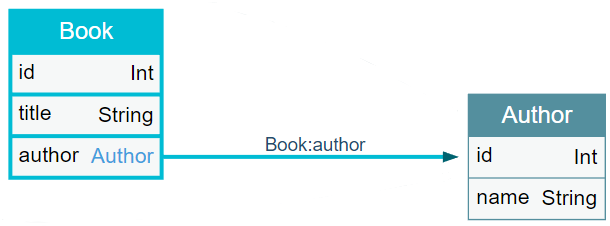
\includegraphics[width=\textwidth,height=\textheight,keepaspectratio]{img/book-author}
\end{center}

Wir nutzen also die Typdefinitionen aus um die Beziehungen zwischen einzelnen Objekten zu bekommen.
Hierbei wird ein Typ dann mit einem anderen Typen verbunden, wenn dieser als Feld im Ursprungstyp vorkommt.
Man muss hierbei klar beachten, dass dies eine gerichtete Beziehung ist.
Eben erstellte Beziehung definiert nur, dass ein Book das Feld Author hat. Wir können nach aktuellem Stand nicht
die Bücher eines Autoren herausfinden da wir diese Kante nicht deklariert haben.
Dies ist allerdings möglich. Definieren wir den Author dann also wie folgt:

\begin{verbatim}
    type Book {
        id: Int
        title: String
        author: Author
    }
    type Author {
        id: Int
        name: String
        written: [Books!]
    }
\end{verbatim}

so ergibt sich folgender, zyklischer Graph:

\begin{center}
    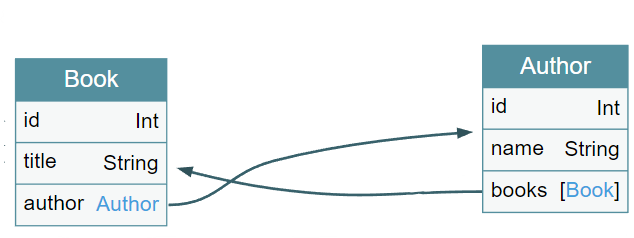
\includegraphics[width=\textwidth,height=\textheight,keepaspectratio]{img/book-author-circle}
\end{center}

\subsection{der komplette Graph}

Wir wissen nun also wie ein GraphQL-Schema einen Graphen repräsentiert und können Algorithmen die auf Graphen funktionieren auch
auf einem GraphQL-Schema anwenden.
Abschließend zu diesem Kapitel sei gesagt, dass es in GraphQL allerdings nicht möglich ist, jeden einzelnen Knoten direkt
abzufragen.
Dies hängt stets von der Definition des Query/Mutation-Types ab, denn alle eingehenden Anfragen müssen vom Query-Type bzw. alle
eingehenden Veränderungen müssen über den Mutation-Type ablaufen.
Der Einfachheit halber werden wir uns jetzt erstmal dem Query-Type widmen.
Jede Anfrage die in GraphQL getätigt werden kann, hat ihren Ursprung im Query-Type.
Somit folgt auch, dass alle Routen stets im Query-Type entspringen müssen.
Dies bedeutet, dass nur Knoten mit Erreichbarkeit vom Query-Type überhaupt abgefragt werden können.
In diesem Beispiel:

\begin{figure}[ht]
    \centering
    \begin{minipage}[b]{0.4\textwidth}
        \begin{verbatim}
    type Query {
        book: Book
        author: Author
    }

    type Book {
        id: Int
        title: String
        author: Author
    }
        \end{verbatim}
    \end{minipage}
    \hfill
    \begin{minipage}[b]{0.4\textwidth}
        \begin{verbatim}
    type Author {
        id: Int
        name: String
        written: [Books!]
    }

    type Publisher {
        name: String
        published:  [Book]
    }
        \end{verbatim}
    \end{minipage}
\end{figure}


wäre es nicht möglich einen Knoten des Publishers abzufragen da dieser Knoten nicht erreichbar ist vom Query-Type.
